\section{Spin-0: radius, torsion and circle scale}

\label{sec:3}

\subsection{Static couplings and radius minimum}

At the round shape and zero twist the scalar potential is

\begin{equation}\tag{S1}\label{eq:S1}
U_0=\frac{\pi^2Lr}{12\kappa^2}(V^2r^2+9\eta^2-36).
\end{equation}

For fixed $L,\eta,V$, a strict positive-radius minimum exists exactly when $V\ne0$ and $\eta^2<4$. Its position and curvature are

\begin{equation}\tag{S2}\label{eq:S2}
r_{\ast}=\frac{\sqrt{12-3\eta^2}}{|V|},
\qquad U_{rr}(r_{\ast})=\frac{\pi^2LV^2r_{\ast}}{2\kappa^2}>0.
\end{equation}

Thus $\eta=V=1$ gives $r_{\ast}=3$. At $V=0$ the potential is linear in $r$: it decreases for $\eta^2<4$, is constant for $\eta^2=4$, and increases for $\eta^2>4$. If $V\ne0$ and $\eta^2\ge4$, it increases for $r>0$ and has no interior minimum. This classification distinguishes zero radial curvature from an actually flat potential. In particular, AX with $\eta=1$ has $U_r=-9\pi^2L/(4\kappa^2)$, despite $U_{rr}=0$.

\begin{figure}[htbp]
\centering
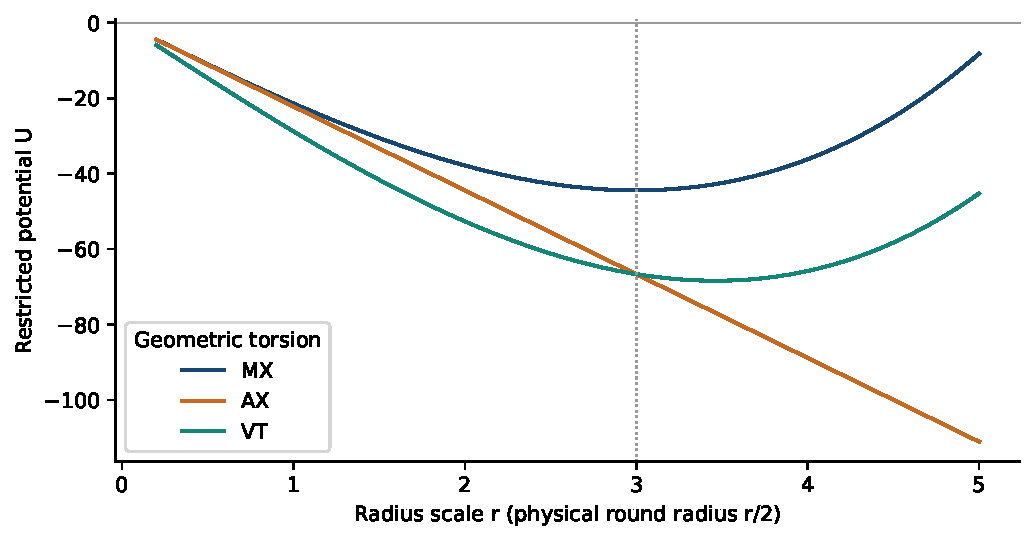
\includegraphics[width=0.93\linewidth]{figures/v3/fig01_radius.pdf}
\caption{Radius potentials at $L=\kappa=1$, with each active torsion coefficient set to one. The MX minimum is $r=3$; the VT minimum is $r=\sqrt{12}$; the AX curve is linear.}\label{fig:fig01_radius}
\end{figure}

The torsion coordinates have positive diagonal static curvature. Their coupling to radius is background dependent:

\begin{equation}\tag{S3}\label{eq:S3}
\begin{aligned}
U_{\eta\eta}&=\frac{3\pi^2Lr}{2\kappa^2},&
U_{VV}&=\frac{\pi^2Lr^3}{6\kappa^2},&
U_{\eta V}&=0,\\
U_{r\eta}&=\frac{3\pi^2L\eta}{2\kappa^2},&
U_{rV}&=\frac{\pi^2Lr^2V}{2\kappa^2}.
\end{aligned}
\end{equation}

Consequently $V$ separates quadratically from $(r,\eta)$ at an AX point with $V=0$, whereas it couples to $r$ in VT and MX. The equality $U_{\eta\eta}=U_{VV}$ at $r=3$ is an equality in these coordinates, not a degeneracy enforced by $SO(3)$. Including $L$ gives further scalar cross terms. Appendix F gives the full gradient and Hessian in one common coordinate system.

\begin{figure}[htbp]
\centering
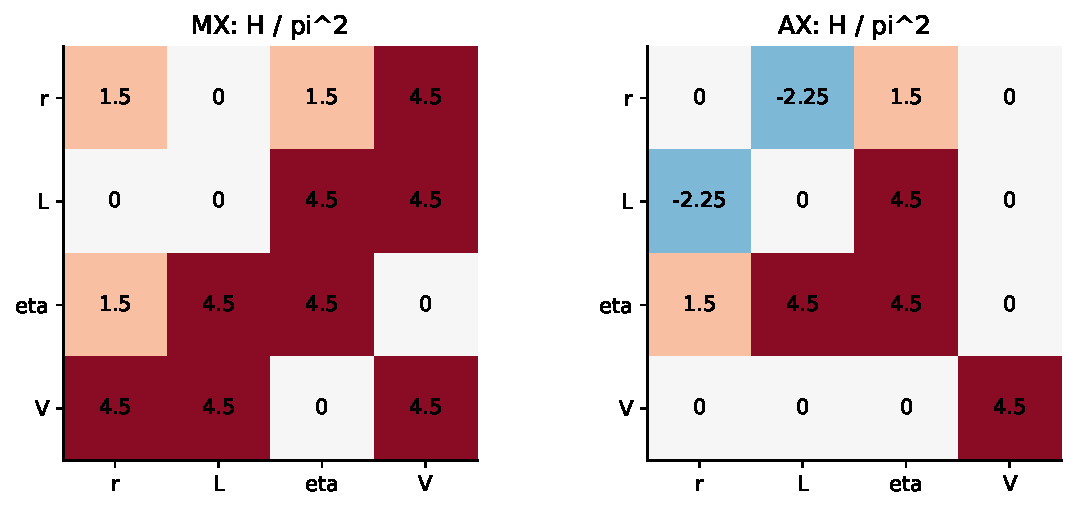
\includegraphics[width=0.93\linewidth]{figures/v3/fig02_scalar.pdf}
\caption{Scalar Hessians in the common coordinates $(r,L,\eta,V)$, divided by $\pi^2$, at the MX point $(3,1,1,1)$ and the AX point $(3,1,1,0)$, with $\kappa=1$. They display couplings between scalar deformations.}\label{fig:fig02_scalar}
\end{figure}

\subsection{Exact scalar action along the circle}

Allow smooth periodic $r(y),L(y),\eta(y),V(y)$, with $r,L>0$, on the round zero-twist coframe. Including the connection derivatives and integrating the total derivatives over the circle gives

\begin{equation}\tag{S4}\label{eq:S4}
\mathcal S_{\mathrm{scalar}}=
\int_0^1dy\left[U_0(r,L,\eta,V)
-\frac{3\pi^2}{4\kappa^2}\frac{r(r')^2}{L}\right].
\end{equation}

Appendix A derives this formula directly from Cartan curvature. Radius carries a circle-derivative term. The $\eta'$ and $V'$ contributions to curvature combine into total derivatives, and no independent $L'$ term remains in the bulk. Here $L(y)$ is the local lapse, while $\int_0^1 L(y)\,dy$ is the circle circumference. Its variation must be specified separately from fixing that circumference. The negative radial derivative coefficient characterizes radial variations of the Euclidean action defined here. The role of lapse and constraints in a canonical formulation is reviewed in \cite{ADM}.

The scalar sector therefore supplies a useful hierarchy: the radius potential at fixed controls, the static response to changing those controls, and the circle-dependent restricted action. For example, the MX radius minimum fixes one derivative to zero, while the remaining scalar gradients need not vanish. This is sufficient for a conditional radius classification and preserves the different roles of size, torsion and circle scale.

In the joint action, scalar changes can couple to shape and twist derivatives through the induced metric (M4). The vanishing of these cross terms in (S4) follows from its round, zero-twist restriction. At nonzero twist the lapse is $\mathcal N$, which differs from the coframe coefficient $L$; an $L'$ cross term in those coordinates need not represent an independent lapse degree of freedom.
